\chapter{Adaptive Informationsverteilung mit RSS und verteiltem Publish/Subscribe}
\label{adapt_informationsverteilung}
Im Folgenden beschreiben  wir eine Methode, ereignisbasierte Informationen an interessierte Klienten zu verteilen. Wir orientieren
uns dabei an RSS. Mit \glqq Ereignis\grqq{} meinen wir im Folgenden eine Informationseinheit (z. B. eine Nachrichten-Schlagzeile),
mehrere Ereignisse k�nnen in einem Datenpaket (RSS-Feed) gesammelt an den Klienten �bermittelt werden. Dazu betrachten wir zun�chst, nach welchem
Schema die Informationen entsprechend dem RSS-System verbreitet werden, zeigen daraus resultierende Probleme auf und schlagen ein Konzept vor,
wie diese Probleme vermieden bzw. verringert werden k�nnen. Auch wenn wir im Folgenden �berwiegend von RSS sprechen, so l�sst sich das Konzept auch auf
andere Informationssysteme �bertragen, die bestimmte Kriterien erf�llen. Je nachdem, auf welche Ebene wir uns beziehen, werden wir entweder von
\glqq Informationen\grqq{} oder \glqq RSS-Feeds\grqq{} sprechen. Das neu entwickelte System wollen wir im Folgenden \glqq \pubsubrss\grqq{} nennen.
 

\subsection{Verteiltes Polling}
Betrachten wir die Gesamtheit der Subscriber und ihr Polling-Verhalten, so erkennen wir, dass aus Sicht eines Servers das Polling-Intervall
dieser Gesamtheit gr��er ist als das Polling-Intervall jedes einzelnen Subscribers. W�nschenswert w�re es, wenn jeder Subscriber von dem
Polling-Intervall der Gesamtheit profitieren k�nnte. Die Idee ist nun, die Subscriber untereinander �ber ein Overlay-Netzwerk zu verbinden,
damit sie sich
gegenseitig die erhaltenen Informationen �bermitteln k�nnen. Das Polling wird also verteilt auf die beteiligten Subscriber. Aber nicht nur das,
wir haben es nun mit einer Kombination aus einem Pull- und einem Push-Ansatz zu tun. Allerdings �bernimmt die Push-Funktion nicht der Server,
sondern die beteiligten Einheiten des Overlay-Netzes, von dem der Server kein Bestandteil ist . Und warum favorisieren wir nicht gleich den
Push-Ansatz bezogen auf den Server? RSS ist ein schon seit l�ngerer Zeit bestehendes Konzept bzw. bestehende Technik.
Dar�ber hinaus ist es weit verbreitet.
Eine Modifikation des Grundkonzeptes w�rde f�r Unternehmen, die es unterst�tzen, bedeuten, bestehende Software austauschen zu m�ssen und
ganz neue Serviceleistungen bereitstellen zu m�ssen. Dies w�rde sicherlich auf Ablehnung sto�en und m�glicherweise nicht die gew�nschte
Verbreitung des neuen Konzeptes mit sich bringen. Ziel ist es, auf dem bestehenden Konzept aufzubauen und es in ein erweitertes Konzept zu
integrieren, um m�glichst f�r den Benutzer als auch f�r den Dienstanbieter ein Minimum an Aufwand zu erreichen. Deolasee et al.
besch�ftigen sich in \cite{bhide02adaptive} mit einer Kombination aus Push-Pull und beschreiben die Probleme, die sich aus reinen Pull- bzw.
Push-Ans�tzen ergeben.

\section{Rolle der Broker}
Broker sind der zentrale Bestandteil des Notifikationssystems. Das Notifikationssystem besteht aus einer Reihe von Brokern,
die untereinander verbunden sind und ein zusammenh�ngendes Netz bilden (Overlay-Broker-Netzwerk, siehe dazu \cite{PietzuchBacon:2003:P2POverlay}).
Ein Broker empf�ngt Feeds von Brokern oder von Klienten/Publishern. Anschlie�end sorgt er f�r eine Verteilung der
Feeds an eine bestimmte Auswahl von mit ihm verbundenen Brokern bzw. Subscribern. Ein Broker kann also eine zentrale Sammelstelle f�r Feeds
unterschiedlicher Anbieter sein. Die einzelnen in den Feeds zusammengefassten Ereignisse k�nnen durch den Broker neu zusammengestellt werden.
Als Kriterien f�r neue Zusammenstellungen bieten sich die Aktualit�t der einzelnen Ereignisse sowie definierbare Filterregeln an. Einzelne 
Ereignisse, die den Broker bereits erreicht haben, brauchen nicht erneut weitergeleitet zu werden und finden daher nach unserem Konzept keinen
Eingang in die neu zusammengestellten Feeds. Dadurch k�nnen Netzressourcen gespart werden. Voraussetzung daf�r ist, dass der Broker einen Cache
unterh�lt, in dem Ereignisse zwischengespeichert werden.\\

Filter k�nnen durch Subscriber definiert und bei Brokern
hinterlegt werden. Aufgrund der Filterregeln k�nnen Ereignisse verschiedener
Anbieter aus den Feeds extrahiert und in einem neuen Feed gesammelt werden. Ein
Subscriber kann also eine individuelle Zusammenstellung der Ereignisse erhalten. Filterregeln und ihre Anwendung wurden schon ausf�hrlich
erforscht und sollen nicht Gegenstand dieser Arbeit sein. Deshalb fanden sie auch keinen Eingang in die weiter unten beschriebene
Simulationsumgebung. Sie erweitern die M�glichkeiten des Systems lediglich, haben aber keinen Einfluss auf das Grundkonzept, um das es hier geht.
Unser System \pubsubrss k�nnte mit bestehenden Pub/Sub-Systemen, welche Filtertechniken unterst�tzen (wie z. B. das System
REBECA \cite{MuFiBu:2001:ArchFrameECommApp}), kombiniert werden.\\

Der folgende Absatz beschreibt Vorg�nge, die eigentlich Teil des jeweiligen Notifikationsdienstes sind, von dem wir abstrahieren. Da jedoch ein
spezifisches Verhalten des Notifikationsdienstes auf eine optimale Funktionsweise des Systems Einfluss nehmen kann, werden wir einige Vorg�nge beschreiben.\\ 
Um sich dem entsprechenden Broker bekannt zu machen und Filter zu hinterlegen, muss sich ein Subscriber bei diesem Broker mit einer speziellen
Registrierungsnachricht registrieren.
Ein Broker braucht nur an diejenigen Subscriber aktuelle Feeds zu �bermitteln, welche auch tats�chlich online sind. Zus�tzlich ist es also notwendig,
dass ein Subscriber in regelm��igen Zeitabst�nden den jeweiligen Broker �ber seinen Online-Status unterrichtet (nennen wir eine solche Nachricht
\glqq KEEPALIVE-Nachricht\grqq{}). Erh�lt ein Broker eine KEEPALIVE-Nachricht eines Subscribers, f�r den er den Zustand \glqq ist offline\grqq{} gespeichert hat,
sollte er diesem eine Zusammenstellung der aktuellsten Ereignisse �bermitteln. Denn kommt es aufgrund von St�rungen im physischen Netzwerk oder
aufgrund von Netz�berlastung zu verloren gegangenen KEEPALIVE-Nachrichten, so gilt der Subscriber f�r seinen Broker als \glqq offline\grqq{}. Dieser wird ihm
daraufhin keine Feeds mehr �bermitteln.
Hat der Subscriber aufgrund von adaptiven Ma�nahmen seine aktuelle Polling-Periode stark angehoben, so wird er zun�chst keine weiteren Feeds beim
entsprechenden RSS-Server selbst�ndig erfragen, so dass ihm eventuell Informationen verloren gehen. Die Menge verloren gegangener Informationen
kann geringer gehalten werden, wenn dem Subscriber die letzten Ereignisse bei Wiedereintritt in das Overlay-Netzwerk als Feed �bermittelt werden.
Entsprechend sollte ein Subscriber seinen jeweiligen Broker dar�ber informieren, wenn er offline geht, um unn�tigen Datentransfer zu vermeiden.\\

Im Zusammenhang mit Brokern werden noch einige weitere Ma�nahmen und Nachrichtentypen notwendig sein, auf die wir jedoch erst in sp�teren Kapiteln zu sprechen
kommen werden, da sie Anpassungen an spezielle Bed�rfnisse darstellen (siehe Kapitel \glqq Churn\grqq{} \ref{cs:churn}) .
%%% Local Variables: 
%%% mode: latex
%%% TeX-master: "diplomarbeit"
%%% End: 

\section{Koordinierung der Subscriber}
\todo{Literaturangaben}\\
\todo{Auflistung der Anforderungen an den Algorithmus}\\
Um das Netz nicht noch zus�tzlich zu belasten, sollte der Overhead, der durch eventuelle Abstimmungsnachrichten entsteht, minimal sein.
Die Konzeption eines Algorithmus sollte unter folgenden Gesichtspunkten geschehen:
\begin{itemize}
  \item Polling durch mehrere bzw. wechselnde Klienten
  \item Anfragen an den RSS-Server sollten nicht gleichzeitig f�r alle Klienten geschehen 
  \item Ausfall von Klienten im Overlaynetzwerk soll Informationsverteilung nicht blockieren
  \item Overhead durch Abstimmungsnachrichten sollte gering gehalten werden
\end{itemize} 
Im Folgenden beschreiben wir einen Algorithmus bzw. eine Technik, die unsere bisher gestellten Anforderungen erf�llt.
\subsubsection{Der Grundlegende Algorithmus}
Die Grundidee ist recht simpel: es sei $t_0$ immer der aktuelle Zeitpunkt. Ausgehend von einem beliebigen Zeitpunkt
$t_x$ mit $t_0\leq t_x$ und einer Intervallspanne $\Delta I$ w�hlt sich jeder Subscriber $i$ innerhalb
des Zeitintervalls $I:=[t_x,t_x+\Delta I]$ einen zuf�lligen Zeitpunkt $TTR_i$ (TimeToRefresh, $TTR$ im allgemeinen), zu dem
er den aktuellen Feed vom RSS-Server erfragt (siehe Abb. \ref{Abb:determine_ttr}).

\begin{picturehere}{3}{1.5}{$TTR$s}{Abb:determine_ttr}
 
\psset{xunit=1cm,yunit=1cm,runit=1cm}
\begin{pspicture}(1.5,-0.5)(7,1)
  \psline{->}(0,0)(7,0)
  \psline{-}(0,0.2)(0,-0.2)
  \uput[0](0,-0.5){$t_0$}
  \psline{-}(3,0.2)(3,-0.2)
  \uput[0](3,-0.5){$t_x$}
  \psline{-}(6,0.2)(6,-0.2)
  \uput[0](6,-0.5){$t_x+\Delta I$}
  \psline{-}(5,0.1)(5,-0.1)
  \uput[0](5,0.4){$TTR_i$}
\end{pspicture}
% \includegraphics{determine_ttr}
\end{picturehere}


Ist $TTR_i$ erreicht, so erfragt Subscriber $i$ den aktuellen Feed vom RSS-Server und setzt nun $TTR_i$ auf einen
Zufallswert innerhalb des
Zeitintervalls $I:=[t_x,t_x+\Delta I]$, wobei $t_x$ ebenfalls neu gew�hlt wird.
Erh�lt Subscriber $i$ vor dem Erreichen des Zeitpunktes $TTR_i$ einen Feed $feed_{new}$ von einem Broker zum 
Zeitpunkt $t_f$ (sei $feed_{old}$ der bisher bei $i$ gespeicherte Feed), so geschieht folgendes:
\pagebreak[3]
\begin{description}
  \item [Fall I:] $feed_{new}$ ist nicht aktueller als $feed_{old}$:
    \begin{description}
      \item keine �nderungen
    \end{description}
  \item[Fall II:] $feed_{new}$ ist aktueller als $feed_{old}$:
    \begin{description}
      \item w�hle $t_x$ neu mit $t_0\leq t_x$
      \item  $TTR_i$ wird gesetzt auf einen Zufallswert innerhalb des Zeitintervalls
        $I:=[t_x,t_x+\Delta I]$
    \end{description}
\end{description}

Die $TTR$s der verschiedenen Subscriber sollten bei der Wahl einer geeigneten Zufallsfunktion �ber $I$ gleichm��ig
verteilt sein. Durch die Wahl eines zuf�lligen Wertes innerhalb von $I$ ist gew�hrleistet, dass nur in extremen Ausnahmef�llen (theoretisch) 
alle Klienten gleichzeitig den RSS-Server kontaktieren.  Nat�rlich kann es vorkommen, dass $TTR$s verschiedener Subscriber auf den gleichen Zeitpunkt fallen
(je nach Gr��e der Intervallspanne $\Delta I$ und der Anzahl der Klienten). Die Verteilung unterliegt jedoch einem kontinuierlichen Wechsel, da die $TTR$s immer
wieder neu berechnet werden. $\Delta I$ bildet eine obere Schranke f�r den erhalt des n�chsten Feeds, da jeder Klient nach sp�testens $\Delta I$ selbst�ndig
den Server kontaktiert, falls in der Zwischenzeit kein aktueller Feed erhalten wurde. Ausf�lle von Klienten k�nnen zwar zu Verz�gerungen beim Erhalt der Feeds
f�hren, sie k�nnen aber die �bermittlung der Feeds zwischen den �brigen Klienten nicht st�ren.\todo{lange �bertragungszeiten}




Gehen wir zun�chst davon aus, es g�be (ausgehend vom aktuellen Zeitpunkt $t_0$) einen Zeitpunkt $nextUpdate$, zu dem der RSS-Server einen neuen Feed bereitstellt.

\section{Angestrebte Dienstg�te: Bevorzugte Polling-Periode}
Bei diesem Ziel gehen wir davon aus, dass jeder Klient sp�testens nach einer von ihm festgelegten Zeitspanne (bevorzugte Polling-Periode) �ber neue Informationen
benachrichtigt werden m�chte. Es wird also eine bestimmte Aktualit�t der Informationen gew�nscht. Sollte dieser Aktualit�tsgrad aufgrund physikalischer Grenzen
(�bertragungs\-zei\-ten, Ser\-ver-Kapazit�t) nicht erreicht werden k�nnen, so sollte der gr��tm�gliche Aktualit�tsgrad erreicht werden. Wir ben�tigen eine Metrik,
um die ``Quality of Service''(Dienstg�te) bestimmen zu k�nnen. Daf�r definieren wir eine Bewertungsfunktion\todo{noch}\\

Bei einigen Sorten von Informationen kann die Aktualit�t der Daten
f�r den Interessenten von entscheidender Relevanz sein, wie z. B. bei aktuellen B�rsennachrichten, wo es f�r den Interessenten darauf ankommt, m�glichst schnell
reagieren zu k�nnen. Dies bei
einem Push-basierten Ansatz erreichen zu k�nnen, ist relativ simpel. Bei �nderung der vom Klienten gew�nschten Informationen �bersendet der Anbieter diese sofort an
alle Interessenten. Nun h�ngt der Aktualit�tsgrad nur von der �bertragungsgeschwindigkeit der Nachrichten im Netzwerk ab. Wir betrachten aber ein Pull-basiertes
System, bei dem erst auf Anfrage der Klienten die angeforderte Information �bersendet wird. Der Interessent hat grunds�tzlich keinen �berblick dar�ber, wann neue
Informationen beim Anbieter vorliegen. Um den gew�nschten Aktualit�tsgrad einer Information zu erreichen, muss ein Klient also sp�testens nach Ablauf der von ihm
bevorzugten Polling-Periode $ppp$ (preferred polling-period) den Server kontaktieren. Der Wert $ppp$ kann von jedem Klienten individuell eingestellt werden.
Bei einer gro�en Anzahl von Klienten im Netzwerk kann dies aber einen
nachteiligen Effekt haben (siehe Abschnitt \ref{vs_ziele}). Steigt die F�llgr��e der Server-Queue, so steigt auch dessen Antwortzeit bez�glich eines Klienten.
Die F�llgr��e der Server-Queue kann nur dann im Mittel konstant gehalten werden, wenn das mittlere Intervall der Ankunftszeiten der Klientenanfragen die mittlere
Bearbeitungszeit pro Anfrage nicht �bersteigt (zu Queueing-Systemen siehe \cite{Kleinrock:Th1975}). Wenn $\lambda$ die mittlere Ankunftsrate der Anfragen ist und
$\bar x$ die mittlere Bearbeitungszeit pro Anfrage, so definieren wir $\rho:=\lambda\bar x$ (utilization factor). Damit die Auslastung der Server-Queue stabil
ist, muss gelten $0\leq\rho<1$ (wir haben es
nach Kleinrock \cite{Kleinrock:Th1975} im allgemeinen mit einem G/G/1-System zu tun, was ein Ein-Server-System bezeichnet, bei dem weder �ber die mittlere
Ankunftszeit noch �ber die mittlere Bearbeitungszeit der Anfragen genaue Aussagen getroffen werden k�nnen). Ist die Kapazit�tsgrenze der Server-Queue erreicht,
werden dar�ber hinaus ankommende Anfragen verworfen. Aber auch diese Nachrichten kosten zun�chst ein gewisses Ma� an Bearbeitungszeit und Netzwerkkapazit�ten.
Eine zu gro�e Rate bzw. Frequenz der Anfragen kann also auch den Aktualit�tsgrad der Informationen senken.\\

\begin{picturehere}{1}{7}{\mbox{Zusammenhang Polling-Rate -- Aktualit�tsgrad}}{Abb:ZshgPollAkt}
 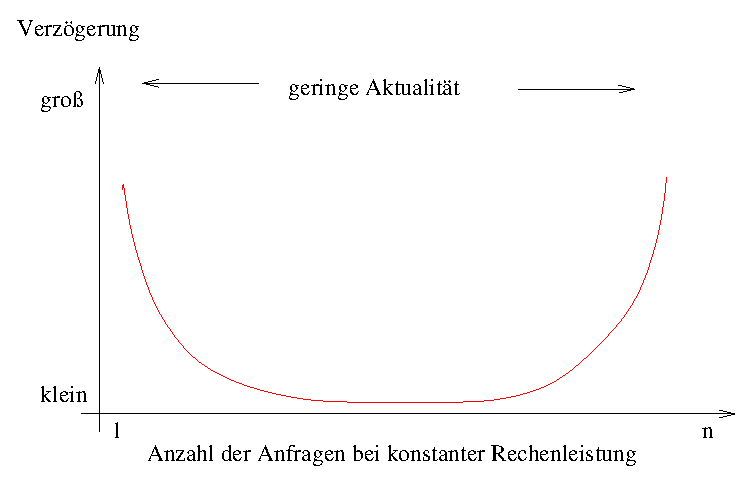
\includegraphics[bb=100 0 200 250,scale=0.9]{Zusammenhang_Pollingrate_Aktualitaetsgrad}
\end{picturehere}

Abbildung \ref{Abb:ZshgPollAkt} zeigt die Auswirkung der Polling-Rate (=1/Polling-Periode) auf den Aktualit�tsgrad der Informationen\footnote{Die Grafik soll
lediglich als schematische Illustration dienen, ein vermeintlicher exponentieller Zusammenhang wurde nicht beobachtet.}.
Solch ein Zusammenhang wurde mit Hilfe der weiter unten beschriebenen Simulationsumgebung validiert.

\paragraph{Wahl der Zufallsspanne:}
Es ist erforderlich, f�r die Berechnung von $\varDelta Z$ eine Gr��e heranzuziehen, welche sich den Gegebenheiten dynamisch anpasst.
$ppp$ ist eine feste Gr��e, bzw.
wird vom Subscriber willk�rlich gesetzt, sollte also nicht ohne weiteres herangezogen werden. Wir definieren die vom Subscriber nicht direkt beeinflussbare
Gr��e $cpp$, welche die aktuelle Polling-Periode bezeichnet, und setzen $\varDelta Z:=cpp$. Bezogen auf $t_x$ wird also sp�testens nach Ablauf der Zeit $cpp$
ein Subscriber seine Anfrage an den RSS-Server stellen. Wie sich $cpp$ im Laufe der Zeit anpassen soll, werden wir im Abschnitt
\ref{css:staukontrolle_pubsubrss} schildern.

\paragraph{Initiale Belegung der aktuellen Polling-Periode:}
Zun�chst stellt sich die Frage, wie $cpp$ initial belegt werden soll, also bei Eintritt des Subscribers in das System.
Die Fragestellung nach einem initialen Timeout ist eine sehr grunds�tzliche, die auch bei anderen Protokollfamilien
eine Rolle spielt (z. B. bei TCP, siehe auch \cite{18216}). Die Problematik ist hier die folgende:
w�hlen wir eine sehr kurze Polling-Periode und treten gleichzeitig viele neue Subscriber dem System bei, so kann es eventuell zur �berlastung
des RSS-Servers kommen. W�hlen wir eine lange Periode, so erh�lt der betreffende Subscriber einen neuen Feed m�glicherweise erst sehr sp�t bzw. zu sp�t.
Wir haben jedoch einen konkreten Richtwert, den $ppp$, und wir w�hlen initial $cpp:=ppp$.
Es stellt sich die Frage, welcher alternative Wert angemessen w�re, da ``kurze Periode'' und ``lange Periode'' relative
Begriffe sind und sich auf die Leistungsf�higkeit des RSS-Servers und auf die Anzahl der Klienten im System beziehen. Beide sind aber bei Einstieg des Subscribers
in das System dem Subscriber noch nicht bekannt.
Jedoch hat der Subscriber ein konkretes Anliegen, n�mlich den Erhalt eines Feeds sp�testens nach der Zeit $ppp$. Also bildet der $ppp$  aus Sicht des Subscribers
den Richtwert. Wie durch die Wahl des $cpp$ auftretende Probleme reduziert werden k�nnen, werden wir in den
Abschnitten \ref{cs:ausbalancierung_der_polling-perioden} und \ref{cs:churn} n�her betrachten.\\

Es gilt also, die aktuelle Polling-Periode $cpp$ eines Klienten in Bezug auf $ppp$ minimal zu w�hlen, so dass die Ungleichung $0\leq\rho<1$ immer noch
erf�llt ist. Es bedarf einer Staukontrolle, die die Auslastung des Servers bestimmt und den Wert $cpp$ entsprechend anpasst.


\todo{Einf�hrung in die Queueing-Theory}

\subsection{Staukontrolle}
Seitdem Computer-Netzwerke explosionsartig an Gr��e und Komplexit�t zugenommen haben, hat sich ein Problem verst�rkt bemerkbar gemacht: Datenstau.
Van Jacobson et. al. \cite{jacobson88congestion} schildern die Beobachtung, dass in der Zeit Mitte der 1980er Jahre Internet-Gateways 10\% der
ankommenden Pakete aufgrund von Puffer�berl�ufen verwarfen. Laut seiner Aussage lag dabei das Problem nicht in den Protokollspezifikationen selbst, sondern
haupts�chlich in deren Implementierungen. TCP (Transmission Control Protocol) ist ein verbindungsorientiertes Transportprotokoll, mit dessen Hilfe der Gro�teil
des Netzwerkverkehrs vonstatten geht. Im Laufe der Zeit wurden in TCP Mechanismen eingebaut und verbessert, um Datenstau festzustellen und soweit wie m�glich
zu vermeiden.\\
\todo{�berleitung}
Auf dem Gebiet der Regelungstechnik besch�ftigt man sich damit, wie eine Gr��e einen bestimmten vorgegebenen Wert erreichen und halten kann. Bei einer Regelung
finden Kontrollmechanismen
Anwendung, um Wertabweichungen festzustellen und auszugleichen.\\

Im Folgenden werden wir Techniken zur Adaption von Werten aus diesen Teilgebieten betrachten und diese auf ihre Tauglichkeit bez�glich der L�sung unseres
beschriebenen Problems untersuchen.
Nicht alle der vorgestellten Techniken sind ohne weiteres auf unsere Problemstellung anwendbar, und wir werden eine L�sung entwickeln, die auf die konkrete
Problemstellung unter Ber�cksichtigung der gegebenen Umst�nde zurecht geschnitten ist.

\subsubsection{Staukontrolle bei TCP}
\label{css:tcp}
TCP (Transmission Control Protocol) ist ein verbindungsorientiertes �ber\-tra\-gungs\-pro\-to\-koll. Es kontrolliert die Daten�bertragung zwischen Sender und
Empf�nger der Endknoten. Dabei wird gew�hrleistet, dass jedes der einzelnen Datenpakete (die einen Datenstrom formen) den Empf�nger erreicht
und die Ordnung der Pakete
innerhalb des Datenstroms bestehen bleibt. Bei Datenstau handelt es sich um Verlust von Datenpaketen. Falls es zu Datenstau kommt, so tritt dieser immer an
Verbindungsknoten (einschlie�lich des Empfangsknotens) auf und kann durch verschiedene Ursachen auf dem Weg zwischen Sender und Empf�nger hervorgerufen werden:
\begin{description}
  \item [Bandbreiten:]
    Unterschiedliche Bandbreiten auf dem Weg zwischen Sender und Empf�nger beeinflussen die �bertragungsgeschwindigkeit einer Verbindung
    nachteilig in der
    Form, dass die ``langsamste'' Leitung (also die mit der geringsten Bandbreite) die
    Gesamt-�bertragungsgeschwindigkeit vorgibt. Trifft eine schnelle Leitung auf eine langsame Leitung, so k�nnen die an der langsamen Leitung ankommenden
    Pakete nicht schnell genug weitergeleitet werden. An diesem Knoten kommt es zum Puffer�berlauf, Datenpakete gehen verloren.
  \item [Anzahl der Verbindungen:]
    An einem Knotenpunkt k�nnen mehrere Verbindungen zusammen kommen, die den Gesamt-Datenfluss an diesem Punkt erh�hen. Auch hier kann es zum Puffer�berlauf
    kommen, so dass Datenpakete verloren gehen.
\end{description}
Damit jedes ausgesandte Paket den Empf�nger erreicht, werden in TCP Best�tigungs-Nachrichten (Acknowledgements, im Folgenden kurz $acks$ genannt) versandt.
Erh�lt der Sender f�r ein gesendetes TCP-Datenpaket kein $ack$, so wird er das Datenpaket erneut senden. Ein wichtiger Bestandteil eines Datenpaketes ist
die Sequenznummer \cite{RFC2581}. Anhand der Sequenznummer kann ein $ack$ eindeutig einem versendeten Datenpaket zugeordnet werden. Innerhalb des $acks$ vermerkt
der Empf�nger ebenfalls, welches Datenpaket er als n�chstes erwartet \cite{RFC793}.
Um eine Staukontrolle zu erreichen wurden einige Algorithmen in TCP integriert (siehe \cite{jacobson88congestion}, wir halten uns dabei an die englischen
Bezeichnungen):
\begin{itemize}
  \item slow-start
  \item round-trip-time variance estimation
  \item exponential retransmit timer backoff
  \item more aggressive receiver ack policy
  \item dynamic window sizing on congestion
  \item Karn's clamped retransmit backoff
  \item fast retransmit
\end{itemize}

Dabei soll erreicht werden, dass die maximal m�gliche Bandbreite (begrenzt durch die minimale Bandbreite (``bottleneck'') auf dem Verbindungsweg, s. o.) voll
ausgenutzt wird, ohne
dass Pakete verloren gehen; es darf also kein Paket in das Netzwerk eingespeist werden, bevor ein altes Paket entfernt wurde (die Verbindung befindet sich dann im
``Equilibrium'', der Paketfluss ist ``conservative'' \cite{jacobson88congestion}). Im Folgenden wollen wir die wichtigsten der oben genannten Algorithmen
vorstellen. Eine genaue Herleitung und Analyse der Algorithmen geht jedoch �ber den Rahmen dieser Arbeit hinaus.
Wir verweisen auf die entsprechenden Quellen in den Literaturangaben.

\paragraph{more aggressive receiver ack policy:}
\footnote{Hier ist in \cite{jacobson88congestion} nicht eindeutig feststellbar,  worauf sich van Jacobson genau bezieht, da er diese Bezeichnung im weiteren Text
nicht mehr verwendet. Es erschien sinnvoll, die folgende im o. g. Text zu findende Erkl�rung diesem Thema zuzuordnen.}TCP
ist ``self-clocking'': da $acks$ erst nach Erhalt der entsprechenden Datenpakete versendet werden k�nnen, bestimmt die Rate der ankommenden $acks$ die
Rate, mit der weitere Datenpakete ausgesendet werden sollen. Die Senderate passt sich somit automatisch der Bandbreite an.

\paragraph{slow-start:}
Durch das ``self-clocking'' tritt nur beim Start des Datentransfers ein Problem auf, da
hier zun�chst eine feste Rate gew�hlt werden muss. Diese wird zu Beginn relativ niedrig gew�hlt, bzw. ein Staufenster ``congestion window'' ($cngw$) 
bestimmt die Anzahl der Pakete pro Sendevorgang. Bei Start des Transfers oder nach Paketverlust wird die Gr��e des Staufenster auf 1 gesetzt.
F�r jedes $ack$ wird das Staufenster um den Betrag 1 erh�ht. Begrenzt wird dessen Gr��e durch das ``advertised receiver window'',
welches vom Empf�nger festgelegt wird und angibt, wieviele Bytes maximal als n�chstes �bersendet werden sollen. Die Zunahme der Gr��e $w$ des
Staufensters geschieht in der Zeit
$rtt\cdot log_2w$, wobei $rtt$ die ``round-trip-time'' des letzten versendeten Datenpaketes ist (Zeit zwischen Versenden eines Datenpaketes und Erhalt des
entsprechenden $acks$). Siehe dazu \cite{jacobson88congestion,RFC2581}. 

\paragraph{round-trip-time variance estimation:}
\label{cssp:tcp_rtt}
$Acks$ k�nnen die Geschwindigkeit des Datenflusses steuern, doch was geschieht, wenn $acks$ aufgrund verloren gegangener Pakete ausbleiben? M�ssen sich
beispielsweise bei voll ausgenutzter Bandbreite pl�tzlich zwei Datenstr�me dieselbe Leitung teilen, kommt es bei gleichbleibender Datentransferrate mit Sicherheit zu
Paketverlusten und somit zu
ausbleibenden $acks$. Der Sender muss einen Timer unterhalten, bei dessen Ablauf das zuletzt gesendete Datenpaket erneut versendet wird (im Folgenden als
Retransmission \todo{anderen Begriff w�hlen: z. B. Wiederholungen}bezeichnet). Paketverlust kann auch
durch Besch�digung der Daten w�hrend der �bermittlung auftreten. Nach van Jacobson \cite{jacobson88congestion} liegt die Wahrscheinlichkeit daf�r aber weit
unter 1\%. Daher lassen Timeouts bei gut eingestellten Timern mit sicherer Gewissheit auf Paketverluste schlie�en \footnote{Zur Problematik
bei Timern siehe \ref{css:timer}}. Diese Timeouts werden pro Verbindung dynamisch berechnet; im Folgenden bezeichnet $rto$ das ``retransmission timeout''-Intervall,
also die Zeitdifferenz bis zum n�chsten Aussenden eines Datenpaketes. Entsprechend der TCP-Spezifikation
berechnet sich dieser Wert wie folgt \cite{18216}:
\begin{equation}
  rto=min\{UBound, max\{LBound, \beta \cdot srtt\}\}
\end{equation}
$\beta$ ist dabei ein empirisch ermittelter Varianz-Faktor, $UBound$ und $LBound$ sind untere und
obere Schranke f�r den $rto$, $srtt$ ist die ``smoothed roundtrip time'' und
wird wie folgt ermittelt:
\begin{equation}
  srtt= \alpha \cdot  srtt+ (1 - \alpha) \cdot  rtt
\end{equation} 
$\alpha$ ist ein ebenfalls empirisch ermittelter Gl�ttungsfaktor (``smoothing factor''). Empfohlene Werte sind f�r $\alpha:$ $0.8 \sim 0.9$ und f�r $\beta:$
$1.3 \sim 2$ \cite{18216}.\\
Laut van Jacobson \cite{jacobson88congestion} liegt hierin folgende Problematik: $\beta$ kann sich h�chstens an eine bis zu 30\% gesteigerte Last anpassen. Aber die
Varianz des Wertes $rtt$ steigert sich rapide mit ansteigender Last. Bei
Laststeigerung �ber die 30\%-Marke hinaus kommt es zu versp�teten $acks$. Der jeweilige abgelaufene Timer bewirkt eine Retransmission des entsprechenden
Datenpaketes, was zu unn�tiger Mehrarbeit des Netzwerkes und zu Bandbreitenverschwendung f�hrt. Daher wird $\beta$ ebenfalls dynamisch berechnet.
Eine Berechnungsmethode findet sich in \cite{jacobson88congestion}.

\paragraph{exponential retransmit timer backoff:}
Um den Datenstau durch mehrfach ausgesandte Pakete nicht noch zu vermehren, muss sich der $rto$ stetig vergr��ern.
Van Jacobson \cite{jacobson88congestion} stellt heraus, dass nur exponentielles Wachstum des $rto$ Erfolg verspricht.
Daher wird nach jedem erneuten Aussenden eines nicht best�tigten Datenpaketes der $rto$ verdoppelt.

\paragraph{dynamic window sizing on congestion:}
Ein Vergr��ern des $rto$ verhindert nur einen zus�tzlichen Datenstau durch erneut ausgesandte Datenpakete. Damit auch die im Anschluss daran neu
ausgesandten Pakete nicht wieder zum Anstieg des Datenstaus f�hren, wird ebenfalls die Gr��e der Staufenster $cwnd$ halbiert (exponentielle Abnahme).
Ausbleibende oder verz�gerte $acks$ geben nur Auskunft �ber auftretenden Datenstau. Sie k�nnen nicht anzeigen, ob die volle Bandbreite einer Verbindung auch wirklich
ausgenutzt wird. Daher sollte die Gr��e der Staufenster nach einem bestimmten Schema angehoben werden. Die Anpassung von $cwnd$ geschieht nach folgendem Prinzip:
\begin{itemize}
  \item Nach jedem Timeout wird $cwnd$ halbiert.
  \item Nach jedem $ack$ f�r neue Daten wird $cwnd$ um $1/cwnd$ erh�ht.
  \item Beim Senden wird das Minimum an Daten von $cwnd$ und dem ``receivers advertised window'' gesendet.
\end{itemize}

Dieser Algorithmus tr�gt zur Stauvermeidung (``congestion avoidance'') bei und besteht parallel zum ``slow-start''-Algorithmus. Van Jacobson gibt in
\cite{jacobson88congestion} ein Auswahlkriterium an, nachdem zustandsabh�ngig zwischen beiden Algorithmen ausgew�hlt wird.

\paragraph{Karn's clamped retransmit backoff:}
\label{csp:karns_algorithmus}
Sequenznummern erm�glichen die Zuordnung eines $acks$ zu dem entsprechenden Datenpaket. Kommt es aufgrund von Timeouts zu Retransmissionen
desselben Datenpaketes, so tritt ein Problem auf, welches Karn und Partridge in \cite{Karn1991} als ``retransmission ambiguity'' bezeichnen:
es kann nicht festgestellt werden, auf welche Aussendung desselben Datenpaketes sich das $ack$ bezieht. Damit ist nicht klar, anhand welches Paketes
sich der $rtt$ bestimmen soll, er wird in jedem Falle nicht verl�sslich sein. Verschiedene Protokollimplementationen behandeln dieses Problem
auf unterschiedliche Weise: teils wird die am l�ngsten zur�ckliegende Aussendung als Grundlage zur Berechnung herangezogen, teils die am k�rzesten zur�ckliegende
Aussendung.\\

Wird die am l�ngsten zur�ckliegende Aussendung  gew�hlt, so k�nnen der $rtt$, damit der $srtt$ und letztlich der $rto$ unverh�ltnism��ig in die H�he schie�en.
In vielen F�llen ist die nachteilige Wirkung nicht besonders gro�, da aufgrund des Datenstaus eine Drosselung der Datentransferrate erw�nscht ist.
Kommt es aufgrund anderer Ursachen zu Paketverlusten (z. B. bei verlustreichen Leitungen durch St�rsignale), so tritt das Gegenteil des gew�nschten Verhaltens
ein: der $srtt$ sinkt auf ein sehr niedriges Niveau, obwohl sich in diesem Falle die Datentransferrate erh�hen sollte.\\

Wird die am k�rzesten zur�ckliegende Aussendung herangezogen, so ist die Wahrscheinlichkeit laut Karn sehr gro�, dass die Zeitfolge zwischen dieser Sendung und dem
ankommenden $ack$ sehr kurz ist, obwohl sich das $ack$ auf eine weiter zur�ckliegende Sendung bezieht. Dies f�hrt zu einer drastischen Reduzierung des $srtt$,
was �berfl�ssige Retransmissionen und damit eine zus�tzliche Verschwendung der Bandbreite zur Folge hat \cite{Karn1991,Jain1986}. Andere Implementationen
lassen die $rtt$ bei Retransmissionen au�er acht. Dies geht gut, solange der $rto$ nicht schneller ansteigt, als der Algorithmus sich adaptieren kann. Ist $\beta$
gut gew�hlt, so ist die M�glichkeit daf�r sehr gering. Tritt dieser Fall dennoch ein, so kommt es (wie im letztgenannten Fall) zu �berfl�ssigen Retransmissionen.\\

Um diesem Problem zu begegnen, schl�gt Karn folgenden Algorithmus vor \cite{Karn1991}:\\
Grunds�tzlich wird der $rto$ nach einem Timeout vergr��ert (``back-off'').
Erreicht ein $ack$ den Sender nach einer Retransmission eines Datenpaketes, so wird keine Neuberechnung des $rtt$ und $srtt$ vorgenommen. Daf�r wird der neu
ermittelte (``backed-off'') $rto$ als Grundlage f�r die n�chste Retransmission bzw. f�r die Aussendung des n�chsten Datenpaketes herangezogen. Nur wenn ein $ack$
den Sender ohne vorausgehende Retransmission erreicht, wird der $rto$ mit Hilfe des nun neu berechneten $srtt$ ermittelt.\\
Die Wahl des neuen $rto$ im Falle einer Retransmission muss laut Karn so erfolgen, dass der $rto$ gr��er ist als die tats�chliche Roundtrip-Time. Typischerweise
geschieht die Steigerung des $rto$ exponentiell (entsprechend des ``exponential retransmit timer backoff'', s. o.).

\paragraph{fast retransmit:}
Erreichen den Sender vier identische $acks$ in Folge, so wird der Sender das vom Empf�nger erwartete Datenpaket sofort aussenden, ohne auf das
Ablaufen des Retransmissionstimers zu warten. ``Slow-start'' wird so lange ausgesetzt, bis ein anderes, nicht zu den vorherigen identisches $ack$ den Sender
erreicht  (\cite{RFC2581}). Die identischen $acks$ lassen sowohl darauf schlie�en, dass ein Datenpaket verloren gegangen ist, als auch, dass andere Datenpakete den
Empf�nger h�chstwahrscheinlich erreichen, da die identischen $acks$ sonst ausgeblieben w�ren. Die den identischen $acks$ zugrundeliegenden Datenpakete beeinflussen
das Datenaufkommen nicht mehr, da diese schon die Empf�nger-Queue erreicht haben. Daher geht man davon aus, dass das erneute, schnelle Senden des fehlenden
Datenpaketes das Netz nicht wesentlich im Negativen beeinflusst. ``Fast retransmit'' sollte, muss aber nicht von einer konkreten TCP-Implementation unterst�tzt
werden.\\

Zus�tzliche Erweiterungen zum TCP in Hinsicht auf hohe Performanz finden sich in \cite{jacobson93tcp}.

\paragraph{Bezug zur Zielsetzung:}
Wie zu Beginn des Abschnittes motiviert, geht es darum, die Auslastung der Server-Queue stabil zu halten, bzw. daf�r zu sorgen,
dass die Ungleichung $0\leq\rho<1$ erf�llt
ist.\\

Zeigen wir zun�chst die Parallelen zwischen unserem Kommunikationsmodell und der Ebene, auf der TCP Anwendung findet: bei unserem Kommunikationsmodell
befinden sich die kommunizierenden Parteien (RSS-Server, Subscriber) ebenfalls an Endknoten. Befindet sich der RSS-Server unter starker Last, so wird seine
Antwort (die �bermittlung des RSS-Feeds) l�nger auf sich warten lassen, als unter geringerer Last. Die Roundtrip-Time zwischen Anfrage und dem vom RSS-Server
�bermittelten Feed (entsprechend einem $ack$) l�sst in gewissem Rahmen auf die Auslastung des Servers schlie�en. Auch in unserem Fall kann die Antwortzeit durch
eine starke Netzbelastung und dadurch verursachte
lange �bertragungszeiten negativ beeinflusst sein. Dies w�rde eventuell unser Ergebnis verf�lschen, da wir nur an der H�he der Serverlast interessiert sind,
die Netzbelastung spielt f�r uns keine Rolle. Um Teill�sungen zu finden, wollen wir aber zun�chst von den Nachrichtenlaufzeiten abstrahieren. Auch in unserem
Fall muss der Subscriber, sollte die Server-Antwort ausbleiben, seine Anfrage erneut senden. Allerdings geschieht die �bermittlung eines RSS-Feeds per HTTP, welches
sich TCP als �bertragungsprotokoll bedient. TCP �bernimmt die Steuerung des Datenflusses, weshalb wir uns um die wiederholte Aussendung von Datenpaketen
nicht zu k�mmern brauchen. In folgenden F�llen ist jedoch das erneute Aussenden von Anfragen bzw. das Herstellen einer neuen TCP-Verbindung notwendig:
\begin{itemize}
\item nach einem Timeout wird die Verbindung unterbrochen, falls keine Reaktion vom Server erfolgt (�berlastung)
\item Verbindung kommt aufgrund einer Server-�berlastung gar nicht zustande (Anfrage findet keinen Eingang in die Server-Queue)
\end{itemize}
F�r diese F�lle sollte der Subscriber ebenfalls einen Timer mitlaufen lassen. Der $rto$ bezeichnet hierbei das Zeitintervall bis zu einem erneuten
Verbindungsaufbau. Wie bei TCP sollte sich der $rto$ stetig vergr��ern, um der Serverbelastung entgegenzuwirken.\\

Alle weiteren �berlegungen werden wir in Abschnitt \ref{css:staukontrolle_pubsubrss} treffen.

\subsubsection{Anwendung eines Regelkreises}
Die Aufgabe einer Regelung besteht darin, bestimmte Gr��en (Temperatur, Spannung, etc.) auf einen
vorgeschriebenen Wert zu bringen und diesen entgegen allen St�reinfl�ssen konstant zu halten (\cite{Bernstein1998}). Bei der Regelung unterscheidet man zwischen
verschiedenen Gr��en, die zusammen einen Regelkreis bilden: 
\begin{description}
  \item [Regelgr��e $x$] oder auch der Istwert: Gr��e, welche konstant gehalten werden soll und zu diesem Zweck erfasst wird
  \item [F�hrungsgr��e $w$] oder auch Sollwert: vorgegebener Wert, auf den die Regelgr��e eingestellt werden soll
  \item [St�rgr��e $z:$] Gr��e, die die Regelgr��e in unerw�nschter Weise beeinflusst
  \item [Regeldifferenz $x_d:$] Differenz zwischen F�hrungs- und Regelgr��e $x_d=w-x$
  \item [Stellgr��e $y:$] Gr��e, durch welche die Regelgr��e in erw�nschter Weise beeinflusst wird
\end{description}

\begin{picturehere}{1}{4}{Regelkreis}{Abb:Regelkreis}
 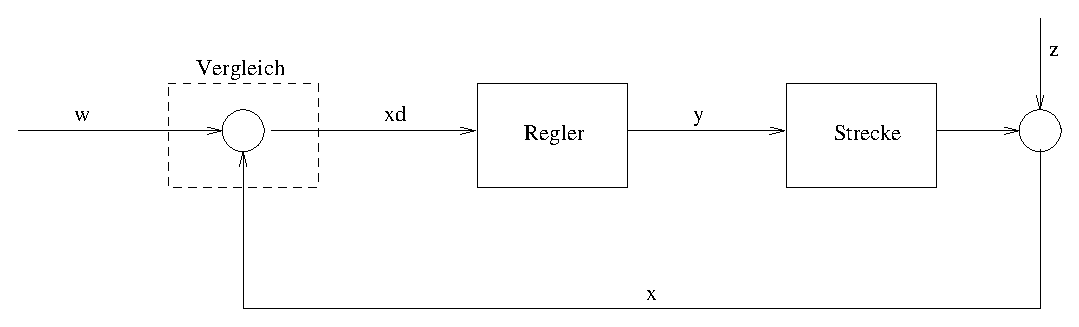
\includegraphics[bb=180 0 682 141,scale=0.75]{Regelkreis}
\end{picturehere}

%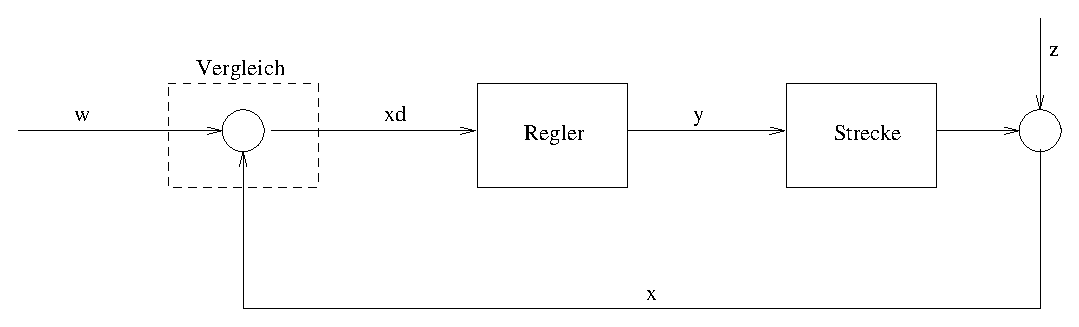
\includegraphics[scale=0.75]{Regelkreis.pstex}

Bild \ref{Abb:Regelkreis} zeigt das vereinfachte Schema eines Regelkreises. Die Regelung basiert auf R�ckkopplung. Bewirkt der Einfluss der St�rgr��e eine
Abweichung der Regelgr��e von der F�hrungsgr��e, so ergibt die Regeldifferenz �ber einen Regler eine Stellgr��e, die entgegengesetzt zur St�rgr��e auf die
Regelgr��e einwirkt. Ziel dabei ist es, die Regeldifferenz auf Null zu bringen.\\
Die Wahl eines geeigneten Reglers h�ngt stark von der Regelstrecke ab. Die Regelstrecke bezeichnet die zu regelnde Anlage oder den zu regelnden Prozess. Wichtig zu
wissen ist, wie die Regelstrecke auf �nderung der Einflussgr��en reagiert. Nach \cite{Bernstein1998} kann man die Regelstrecken grob durch folgende Merkmale 
unterscheiden:
\begin{itemize}
  \item Regelstrecken mit und ohne Ausgleich
  \item Regelstrecken mit und ohne Totzeiten bzw. Zeitgliedern
  \item lineare oder nichtlineare Regelstrecken
\end{itemize}

Bei Regelstrecken mit Ausgleich erreicht die Ausgangs- bzw. Regelgr��e nach einer gewissen Zeit einen stabilen Zustand (Bsp. Raumtemperatur). Existiert kein
stabiler Zustand (Regelstrecke ohne Ausgleich), so �ndert sich bei konstanter Eingangs- bzw. Stellgr��e die Regelgr��e mit
konstanter Geschwindigkeit oder Beschleunigung (Bsp. F�llen eines Wasserbeh�lters). Totzeit bezeichnet eine Zeitverz�gerung, bis sich die �nderung der Stellgr��e
auf die Regelgr��e bemerkbar macht. Bei linearen Regelstrecken folgt die Regelgr��e der Stellgr��e proportional.

Meist liegt eine Kombination dieser Eigenschaften vor. Um die Stellgr��e entsprechend der Regeldifferenz anzupassen, wird ein Regler ben�tigt.

\paragraph{PID-Regler:}
Ein PID-Regler ist ein allgemeiner Reglertyp, der h�ufig f�r Regelungen Verwendung findet. Er ist eine Kombination aus einem P-, einem I- und einem D-Regler.
Ein P-Regler sorgt daf�r, dass (im station�ren Zustand) ein dem Eingangssignal proportionales Ausgangssignal geliefert wird (unter Zuhilfenahme eines
Verst�rkungsfaktors). Ein I-Regler summiert die Regeldifferenz �ber einen gewissen Zeitraum und f�hrt damit eine Integration aus. Je l�nger eine Regeldifferenz
besteht, desto gr��er wird die Stellgr��e. Ein D-Regler reagiert nur auf die �nderungsgeschwindigkeit der Regeldifferenz. Er liefert einen entsprechend starken,
kurzen positiven Impuls \todo{soll weg:(ein reiner D-Regler hat in der Praxis keine Bedeutung)}.

Die allgemeine mathematische Gleichung f�r einen PID-Regler lautet wie folgt
(siehe \cite{WBuettner1991}):
\begin{equation}
  u(t)=K_R\left[\quad e(t) \quad + \quad
    \frac{1}{T_I}\int\limits_{0}^{t}e(\tau)d\tau \quad + \quad
    T_D\frac{de(t)}{dt} \quad \right]
\end{equation}

Die einzelnen Gr��en sind:
\begin{description}
  \item [$u(t)$] Stellgr��e
  \item [$e(t)$] Regeldifferenz
  \item [$K_R$] Verst�rkungsfaktor
  \item [$T_I$] Integrationskonstante
  \item [$T_D$] Differentiationskonstante
\end{description}

Es werden nicht f�r alle Regelungen alle Anteile ben�tigt. Durch Weglassen der entsprechenden Anteile erh�lt man die Regler P, PI bzw. PD. Reine P-Regler finden
nur Verwendung bei Regelstrecken linearen Verlaufs. Doch selbst hier zeigt sich, dass bei Regelabweichungen, die durch eine St�rgr��e hervorgerufen werden, die
St�rgr��e lediglich in ihrer Wirksamkeit gemindert werden kann. Eine vollst�ndige Beseitigung tritt nicht ein, da die Regelabweichung selbst notwendig ist, um eine
Verstellung des Stellgliedes vorzunehmen \cite{Bernstein1998}. Mit einem I-Regler kann man die Regelabweichung sehr genau unterbinden, jedoch arbeitet dieser
relativ langsam und neigt zu Schwingungen. Die Vorteile beider Reglertypen vereint der PI-Regler. Reine D-Regler finden in der Praxis keine Verwendung, da sie bei
stabiler Regelgr��e nicht in den Regelvorgang eingreifen k�nnen. Die Kombination mit einem P-Regler (also ein PD-Regler) bewirkt ein schnelleres Anspringen der
Regelung bei pl�tzlicher Regelabweichung im Vergleich zu einem reinen P-Regler.\\

\paragraph{Bezug zur Zielsetzung:}
Wir k�nnen die Erf�llung der Ungleichung $0\leq\rho<1$ durch einen Regelkreis beschreiben. Die zu regelnde Gr��e ist dabei $\rho$. Die Stellgr��e
ist $cpp$. Aus Sicht eines Klienten
sind die $cpp$s der �brigen Klienten eine St�rgr��e, da ihre Ver�nderung die Auslastung des Servers beeinflusst. Bei der Regelstrecke handelt es
sich im Allgemeinen um einen nicht-linearen Typ mit Ausgleich und Totzeit. Als Regler sollten wir daher einen PI-Regler verwenden. Eine differentiale Eigenschaft
wollen wir zun�chst au�er Acht lassen, da diese nur zur Feinabstimmung beitr�gt.\\

Um $\rho$ messen zu k�nnen, muss der Regler einen direkten Zugriff auf die Werte $\lambda$ und $\bar x$ (s.o.) erhalten k�nnen.
Dies ist aber im Allgemeinen bzw. bei unserem
favorisierten Ansatz nicht m�glich, da nur der Server diese Werte ermitteln kann und diese entsprechend des Konzeptes nicht an die Klienten �bermittelt.
Ein Klient kann somit nur aufgrund anderer Indizien auf diese Werte r�ckschlie�en.
Das einzige Indiz ist das Antwortverhalten bzw. die Antwortzeit des Servers auf eine Anfrage des Klienten. Abstrahieren wir von den Nachrichtenlaufzeiten,
so l�sst eine lange Antwortzeit des Servers auf einen gewissen �berlastungsgrad schlie�en. Mit Hilfe der $rtt$ k�nnen wir somit die $cpp$ bestimmen, also
$cpp=f\cdot rtt$, wobei $f$ ein beliebiger Faktor ist (proportionaler
Anteil des Reglers). Eine konstante Abtastrate w�re w�nschenswert, damit ein Regler zu jedem
Zeitpunkt die gleiche Reaktionszeit zeigen kann. Falls wir nur mit den regul�ren Anfragen nach RSS-Feeds zur Bestimmung der Server-Antwort arbeiten,
bewirkt eine Drosselung des $cpp$ ebenfalls eine Drosselung der Abtastrate.
Man k�nnte die Reaktionszeit des Servers anders ermitteln, z. B. durch konstantes Anpingen (z. B. mit Hilfe des Kommandos ``ping'').
Dies h�tte jedoch u. a. zur Folge, dass dadurch bei einer gro�en Anzahl Klienten im Overlay-Netzwerk ebenfalls
eine Server-�berlastung erreicht werden k�nnte. Die Beobachtung der zu regelnden Gr��e w�rde diese also gleichzeitig beeinflussen. Au�erdem erreicht ein Ping
nicht die Anwendungsschicht des Servers, eine �berlastung auf dieser Ebene bleibt eventuell unbemerkt. Des Weiteren kann es vorkommen,
dass eine Anfrage eines Klienten bei voller Queue vom Server verworfen wird. Eine Server-seitige Antwort wird in diesem Fall ausbleiben. Nach einem
Timeout muss also der Klient seine Anfrage erneut stellen. Ist dieses Timeout konstant und relativ klein, so kann dies ebenfalls zu einer Mehrbelastung des Servers
f�hren. Hierbei kommt das f�r den Regler erforderliche Ereignis (Server-Antwort) gar nicht zustande, somit kann eine Regelung �ber den Regler gar nicht in der
gew�nschten Weise stattfinden. Das Indiz f�r eine gesteigerte Server-Belastung ist hier also eine Negativ-Nachricht: das Ausbleiben der Server-Antwort. Um die
Mehrbelastung des Servers in diesem Fall einzud�mmen, k�nnen wir die Timeouts und somit die $ccp$ je nach Zeitdauer vergr��ern (integrativer Anteil,
vgl. Abschnitt \ref{css:tcp}).\\

Es zeigt sich, dass das Konzept des PID-Reglers nur modifiziert anwendbar auf unsere Problemstellung ist.
Wie schon angedeutet, werden wir die Grundideen eines PID-Reglers in unserer hergeleiteten Methode wiederfinden.

\subsubsection{Grunds�tzliches zu Timern}
\label{css:timer}
\todo{folgt}

\subsubsection{Staukontrolle bei Pub/Sub-RSS}
\label{css:staukontrolle_pubsubrss}
Wir fassen kurz zusammenfassen, welche prim�ren Ziele und damit verbundenen sekund�ren Ziele wir verfolgen: grunds�tzlich geht es um die Bestimmung des Wertes
$ttr$ eines Subscribers (siehe Abschnitt \ref{cs:der_grundlegende_algorithmus}).
Zur Erinnerung: $ttr$ bezeichnet ``Time-To-Refresh'', also den konkreten Zeitpunkt, zu dem die n�chste Anfrage an den jeweiligen RSS-Server
gestellt werden soll. Um $ttr$ zu bestimmen ben�tigen wir $\varDelta ttr$. Ein wichtiger Parameter zur Bestimmung von $\varDelta ttr$ ist der $cpp$. Um einer
l�ngerfristigen
�berlastung des RSS-Servers entgegenzuwirken, muss der $cpp$ eines Subscribers entsprechend der Serverbelastung angepasst werden.
Wir m�ssen also ein Ma� f�r die Serverbelastung bestimmen, was auch bei uns die ``Roundtrip-Time'' sein soll, also die Zeit, die zwischen Aussendung
einer Anfrage und dem Erhalt des entsprechenden Feeds vergeht. Die Roundtrip-Time ist jedoch nicht immer eindeutig zu bestimmen.
Im Folgenden soll der Wert $rtt$ den N�herungswert an die Roundtrip-Time bezeichnen, den es gilt
zu berechnen. Mit Hilfe von $rtt$ k�nnen wir dann $rto$ und $cpp$ ermitteln.\\

Der konzeptionelle Unterschied zwischen $rto$ und $cpp$ ist folgender: w�hrend der $cpp$ zur Berechnung des $\varDelta ttr$ bei erfolgreicher Anfrage
(also nach Erhalt eines RSS-Feeds) dient, \todo{dient,dient}dient der $rto$ zur Berechnung des $\varDelta ttr$ bei nicht erfolgreicher Anfrage, also nach Ablauf des
``Retransmission-Timers'' ohne Erhalt eines
RSS-Feeds. Ob wir diese Werte separat berechnen, oder ob wir einen funktionalen Zusammenhang zwischen diesen Werten herstellen, werden wir im Folgenden er�rtern.

Bei TCP gibt es ebenfalls eine funktionale Unterscheidung zwischen $srtt$ und $rto$,
wobei der $cpp$ hier f�r den $srtt$ bei TCP steht. Im Unterschied zu TCP reicht bei uns der Wert $cpp$ als Timeout \todo{siehe Korrektur}f�r die n�chste Anfrage
jedoch nicht aus, da es in unserem Fall
nicht um einen Datenstrom \todo{ANPASSUNG AN TCP}und somit nicht um die Aussendung des n�chsten Datenpaketes geht. In unserem Fall muss die Zeit
bis zum Aussenden der n�chsten Anfrage $\varDelta ttr$, die sich mit Hilfe von $cpp$ berechnet, ermittelt werden.\\

Beim Anpassen des $cpp$ m�ssen wir ber�cksichtigen, dass grunds�tzlich nicht ein Subscriber alleine f�r eine �berlastung verantwortlich ist, sondern in den
meisten F�llen eine Menge von Subscribern, die gemeinsam auf den gleichen RSS-Server zugreifen. Eine Senkung des $cpp$ kann also eine drastische Wirkung haben,
da je nach Verfahren diese Ma�nahme eventuell jeder beteiligte Subscriber ergreift.\\

Zur Berechnung des $rtt$ m�ssen wir die RSS-Feeds nach ihrem Ursprung unterscheiden: Feeds, die ein Subscriber von einem Broker erh�lt, m�ssen anders behandelt
werden als Feeds, die von einem RSS-Server ausgesandt werden. F�r die Berechnung des $rtt$ spielen nur diese Feeds eine Rolle, da nur diese Auskunft �ber eine
eventuelle Server-Belastung geben k�nnen.\\

Wir haben uns in den vorhergehenden Abschnitten m�gliche Techniken zur Staukontrolle und -vermeidung bei TCP und bei der Regelungstechnik angesehen
und dabei festgestellt, dass die dort beschriebenen L�sungsans�tze nur bedingt auf unser Problem anwendbar sind.
Im Folgenden wollen wir eine L�sung aufgrund einer problemorientierten Sichtweise konzipieren und dort Bez�ge zu den beiden anderen Konzepten herstellen,
wo es angebracht erscheint.\\

Wie schon erw�hnt �bernimmt bei einer Anfrage an einen RSS-Server die TCP-Schicht die  Datenfluss- und Staukontrolle, so dass wir uns an dieser Stelle
nicht um wiederholte Aussendungen von Anfragen zu k�mmern brauchen. Wird die Verbindung jedoch unterbrochen bzw. kommt sie gar nicht zustande, so muss die
Klienten-Software den Verbindungsaufbau nach einer gewissen Zeit wiederholen. Die Zeit, die in diesem Fall bis zum n�chsten Verbindungsaufbau vergehen soll,
wird durch $rto$ bestimmt. Das Problem der ``retransmission-ambiguity'' (siehe \ref{csp:karns_algorithmus}) kann nicht eintreten. Soll ein Verbindungsaufbau zu
einem RSS-Server geschehen, so sprechen wir im Folgenden der Einfachheit halber von der Aussendung eines ``Feed-Requests''.\\
Erh�lt ein Subscriber
einen Feed, so muss in jedem Fall der $ttr$ f�r die Aussendung des n�chsten Feed-Requests berechnet und ein entsprechender
Timer $RQT$ (f�r ``Request-Timer'') eingerichtet werden, nach dessen Ablauf der Feed-Request versendet wird. Nach Aussendung des Feed-Requests muss nun ein
Timer $RT$ (f�r ``Retransmission-Timer'') eingerichtet werden, nach dessen Ablauf der Feed-Request erneut ausgesandt wird. Die Unterscheidung der beiden Timer
ist rein konzeptioneller Natur, in der Praxis k�nnen wir sagen: $RT:=RQT$, der $RQT$ wird dann je nach Situation unterschiedlich gesetzt. Um eine klarere
Differenzierung vorzunehmen, werden wir trotzdem dort zwischen den Begriffen $RQT$ und $RT$ unterscheiden, wo es der Deutlichkeit halber angebracht erscheint.
Mitbestimmend f�r den $RQT$ ist der $cpp$, mitbestimmend f�r den $RT$ der $rto$. $cpp$ wird ebenfalls je nach Situation unterschiedlich berechnet.\\

Eine untere Schranke f�r den Wert $cpp$ soll $ppp$ bilden. Da jeder Subscriber $ppp$ individuell festlegen kann, ist es nicht notwendig,
$cpp$ kleiner als $ppp$ zu w�hlen.
Das hei�t nicht, dass ein Subscriber fr�hestens nach Ablauf der Zeit $ppp$ einen neuen Feed bekommt: existieren im gleichen Netzwerk andere Subscriber, die einen
niedrigeren $ppp$ eingestellt haben, so kann jener Subscriber davon profitieren, da ihm dann ebenfalls neu auftretende Feeds nach k�rzerer Zeit zugestellt werden.
M�chte ein Subscriber sicher gehen, dass ein bestimmter Aktualit�tsgrad der Feeds erreicht wird, so muss er den $ppp$ entsprechend setzen.\\

Wir wollen ebenfalls eine obere Schranke f�r den Wert $cpp$, den $mpp$ (f�r maximale Polling-Periode), definieren. Dieser vermeidet, dass bei ung�nstigen
Konstellationen der $cpp$ zu gro� wird (z. B. wenn jeder Feed-Request eines Subscribers vom RSS-Server verworfen wird, obwohl der Server nicht stark
�berlastet ist). Dieser sollte abh�ngig vom jeweiligen Overlay-Netzwerk bestimmt werden.\\

Der $rtt$ kann nur gemessen werden, wenn ein Subscriber einen RSS-Feed von einem RSS-Server zugesandt bekommt. Grunds�tzlich dient der Wert $rtt$ als
Bezugspunkt f�r $cpp$. Bei jeder �nderung von $rtt$ berechnet sich $cpp$ wie
folgt:
\begin{equation}
  cpp:=min\{mpp,max\{rtt,ppp\}\}
\end{equation}
Bei Einstieg des Subscribers in das System wird (s. o.) $rtt:=ppp$ gesetzt. Erh�lt ein Subscriber einen RSS-Feed vom RSS-Server, so wird,
falls der $RT$ bisher noch nicht abgelaufen ist, $rtt$ auf die gemessene Roundtrip-Time gesetzt.
Bestimmend f�r den $RT$ ist der $rto$, welcher initial und bei Erhalt eines vom RSS-Server direkt versendeten Feeds auf $rto:=cpp$ gesetzt wird.
Bei jeder Aussendung eines Feed-Requests wird
zun�chst der $rto$ verdoppelt und $RT$ neu gesetzt. Dies bedeutet exponentielles Wachstum des $rto$. Damit das System skalierbar ist und die Adaption auch bei
gro�en Netzen noch in angemessener Zeit geschieht, muss die
Anpassung exponentiell erfolgen (siehe ``exponential retransmit timer backoff'' in Abschnitt \ref{css:tcp}).\\
Erh�lt ein Subscriber einen RSS-Feed von einem RSS-Server, so muss die Roundtrip-Time bestimmt werden. Der Inhalt des Feeds erreicht den Subscriber aufgrund der
auf einer tieferen Ebene liegenden TCP-Schicht als Datenstrom. Hierbei k�nnen wir die Zeit zwischen Verbindungsaufbau und erstem erhaltenen Byte messen,
um die Roundtrip-Time zu bestimmen, welche durch den Wert $rtt$ festgehalten wird.
Muss es allerdings zu mehrfachen Versuchen kommen, eine Verbindung aufzubauen, so reicht diese gemessene Roundtrip-Time f�r die Besimmung von $cpp$ nicht aus.
Die Notwendigkeit mehrfacher Versuche l�sst auf eine �berlastung des Servers schlie�en, so dass der $cpp$-Wert entsprechend angepasst werden muss. Daher soll
$rtt$ nicht die eigentliche Roundtrip-Time bezeichnen, sondern in $rtt$ m�ssen die mehrfachen Verbindungsversuche mit einflie�en. Bezeichne $t_{V_1}$ den Zeitpunkt
des ersten Verbindungsversuches und $t_B$ den Zeitpunkt des ersten auftretenden Datenbytes, so bestimmt sich $rtt$ wie folgt:

\begin{equation}
rtt:=t_B - t_{V_1}
\end{equation}

Letztlich wird also

Hier kann man eine Analogie zum Konzept der PI-Reglern herstellen (obwohl es nur Parallelen in den Grundideen gibt): w�hrend man den bereits berechneten $cpp$
als proportionalen Anteil in der Berechnung auffassen kann, gibt es eine Parallele zwischen der Anpassung des $rto$ und dem integrativen Anteil beim PI-Regler,
da die Anpassung des $rto$ die zeitliche Dauer der Server-Antwort ber�cksichtigt.\\

Ein Varianzfaktor wird hierbei nicht hinzugezogen. Berechnungen auf dieser Grundlage
lieferten in der Simulation gute Ergebnisse. Eine Optimierung w�re eventuell m�glich, wenn man einen Varianzfaktor entsprechend der $rto$-Berechnung bei
TCP hinzuzieht. Dies soll aber nicht Gegenstand dieser Arbeit sein und bleibt offen f�r weitere Forschungen.
Neuberechnungen von $cpp$ und $rtt$ finden zun�chst nur dann statt, wenn ein Subscriber einen RSS-Feed von einem RSS-Server erh�lt.
Weitere Verbesserungen werden wir in Abschnitt \ref{cs:ausbalancierung_der_polling-perioden} betrachten.\\

\paragraph{Ungenauigkeiten und Probleme:}
Wie oben angedeutet, entspricht der gemessene $rtt$, auch wenn der $RT$ noch nicht abgelaufen ist, nicht immer der tats�chlichen Roundtrip-Time.
Denn denkbar ist folgendes
Szenario: aufgrund abgelaufener Retransmissionstimer hat ein Subscriber einige Feed-Requests mehrfach ausgesandt. Diese sind aber nicht verloren gegangen, sondern
befinden sich in der Queue des RSS-Servers, welcher einer zeitgerechten Antwort nicht nachkommen kann. Der erste vom Server ausgesandte Feed dient als
Berechnungsgrundlage f�r den $rtt$ des Subscribers, welcher nach kurzer Zeit (nach Ablauf von $RQT$) eine neue (erste) Anfrage stellt. Sendet ihm nun der RSS-Server
einen Feed aufgrund eines noch in der Queue befindlichen Feed-Requests, so interpretiert der Subscriber jenen als Antwort auf seine letzte Anfrage, obwohl er sich
noch auf die vorherige Anfrageserie bezieht. In diesem Falle ist der $rtt$ falsch. Dieses Problem lie�e sich nur beheben, wenn die Feeds den Feed-Requests
eindeutig zuordenbar w�ren (z. B. durch Sequenz- und Retransmissions-Sequenznummern). Da unser Ansatz dies nicht zul�sst, m�ssen wir diese eventuelle Ungenauigkeit
leider in Kauf nehmen.\todo{siehe Korrektur}\\

Ein Problem ist denkbar, welches sich auch in der Simulation gezeigt hat: einige wenige Subscriber, welche Anfragen mit einer hohen Frequenz aussenden (also
bei einer sehr kleinen Polling-Periode), k�nnen die �brigen Subscriber ``aussperren''. Die Subscriber, welche eine k�rzere Polling-Periode berechnet haben, k�nnen
diese halten, da ihre Anfragen (bedingt durch deren Menge) eine gr��ere Chance haben, in der Server-Queue zu landen. Die Queue wird unter diesen wenigen
Subscribern aufgeteilt. Somit erhalten sie die Feeds als Antwort auch mit einer h�heren Frequenz vom Server. Dabei muss man bedenken,
dass sich die Anfragen mehrfacher Retransmissionen in der Server-Queue befinden k�nnen. Diese werden
nach und nach bearbeitet, Feeds werden an den jeweiligen Subscriber geschickt. Eine eventuelle Messung der Roundtrip-time wird dadurch verf�lscht, so dass der
Subscriber (in der Annahme, der Server kann der Beantwortung einer Anfrage schnell nachkommen) seinen $cpp$ konstant halten kann. Die Polling-Perioden der
�brigen Subscriber wachsen dagegen drastisch. Denn gerade durch den Umstand, dass ihre
Anfragen seltener in der Server-Queue landen, werden sie durch die daraufhin verz�gerten (oder ausbleibenden) Antworten ihre Polling-Perioden vergr��ern.
Dieser R�ckkopplungseffekt f�hrt dazu, dass ihre Polling-Perioden dauerhaft gro�e Werte aufweisen und f�r diese Subscriber kaum Chancen bestehen,
Feeds vom Server zu erhalten. Nat�rlich bekommen diese Subscriber ebenfalls die Feeds �ber das Netzwerk zugesandt. Die Polling-Perioden der verschiedenen Subscriber
sind aber stark auseinander gerissen, sie befinden sich in Dysbalance, wobei keine �nderungen der Polling-Perioden mehr zu erwarten sind.
Verlassen nun die Subscriber mit einer kurzen Polling-Periode das Netz, so steht dieses
zun�chst fast still, da die restlichen Subscriber Anfragen erst nach einer gro�en Zeitdifferenz erneut aussenden. Wie man dieser Dysbalance entgegenwirken kann,
werden wir in Abschnitt \ref{cs:ausbalancierung_der_polling-perioden} darstellen.\\

Ein \label{cssp:ung_u_probl:dysbalance} weiterer eventuell problematischer Punkt (im obigen Absatz bereits angesprochen) ist die Berechnung des Wertes $rtt$,
falls $RT$ noch nicht abgelaufen ist. In diesem Fall wird bei unserer Berechnung
der $rtt$ direkt auf die gemessene Roundtrip-Time gesetzt, w�hrend bei TCP diese nur zum Teil (unter zus�tzlicher Zuhilfenahme des Gl�t\-tungs\-fak\-tors $\alpha$,
siehe Abschnitt \ref{cssp:tcp_rtt}, Seite \pageref{cssp:tcp_rtt}) in die Berechnung eingeht. Diese direkte R�ck\-setzung k�nnte zu einem starken Schwingungsverhalten der
Server-Belastung und somit der Polling-Perioden im System f�hren. Allerdings ist eine schnelle Reaktion des Systems auf eine
verbesserte Server-Reaktionsf�higkeit erw�nscht, und in der Mehrheit der F�lle werden nicht alle Subscriber gleichzeitig den Wert $rtt$ auf diese Weise ermitteln.
Beobachtungen zeigen jedoch, dass es bei einer pl�tzlichen Erreichbarkeit des Servers tats�chlich zu einem Ansturm
auf diesen kommen kann. Wir werden aber
dieses Ph�nomen in Zusammenhang mit der vorgestellten Technik in Abschnitt \ref{cs:ausbalancierung_der_polling-perioden} eind�mmen k�nnen. 


%%% Local Variables: 
%%% mode: latex
%%% TeX-master: "diplomarbeit"
%%% End: 

\subsection{Feeds und Timer}
\label{css:feeds_und_timer}
Bisher sind wir noch nicht weiter darauf eingegangen, welche ausl�senden Faktoren f�r das Setzen der Timer $RT$ und $RQT$ verantwortlich sind. Wir haben nur den
Timer $RT$ n�her betrachtet: ausl�sendes Ereignis ist die Aussendung eines Feed-Requests an den RSS-Server. Das Setzen des Timer-Intervalls $rto$ erfolgt wie im
vorherigen Abschnitt besprochen.\\

Bleibt zu bestimmen, wann und wie $RQT$ gesetzt wird. Erh�lt ein Subscriber einen RSS-Feed, so muss er bestimmen, wann der n�chste Feed-Request an den RSS-Server
gesendet werden soll. Dazu m�ssen wir einen erhaltenen Feed nach Aktualit�t und Herkunft unterscheiden. Erh�lt ein Subscriber einen neueren Feed von einem
Broker oder von einem RSS-Server, so
m�ssen $\varDelta Z$ und $t_x$, also $\varDelta ttr$, in Abh�ngigkeit von den enthaltenen Events entsprechend der in Abschnitt \ref{cs:der_grundlegende_algorithmus}
beschriebenen Methode neu bestimmt werden: f�r jeden RSS-Server\todo{MEHRZAHL AUFL�SEN;SIEHE KORREKTUR}, auf den sich ein neues Event bezieht, m�ssen diese Werte
neu berechnet und der entsprechende $RQT$ neu gesetzt werden. Erh�lt ein Subscriber dagegen einen Feed von einem Broker ohne neue Informationen,
so bleibt der laufende $RQT$ bestehen, denn dies ist genau jener Fall, in welchem es in der Verantwortung des Subscribers liegt, in K�rze hinzukommende
Ereignisse zu entdecken. Bei Erhalt eines Feeds von einem RSS-Server ohne neue Informationen muss $RQT$
neu gesetzt werden, denn es ist davon auszugehen, dass dem Feed ein Feed-Request aufgrund eines abgelaufenen $RQT$ vorausgegangen ist.
Dabei wird das $RQT$-Intervall auf $cpp$ gesetzt, $\varDelta Z$ wird nicht neu berechnet und $t_x$ wird auf $t_x:=t_0+cpp$ gesetzt.\\

Das ganze als algorithmisches Beispiel in einer an Java angelehnter Pseudonotation:

\begin{verbatim}

aktualisiere_RQT_durch_alten_Brokerfeed {
}

aktualisiere_RQT_durch_neuen_Brokerfeed {

    berechne_delta_ttr(cpp);
    setze_RQT(delta_ttr);

}

aktualisiere_RQT_durch_alten_Serverfeed {

    berechne_rtt();
    setze_cpp(rtt);
    stoppe_RT();
    setze_rto_zur�ck();
    setze_RQT(cpp);

}

aktualisiere_RQT_durch_neuen_Serverfeed {

    berechne_rtt();
    setze_cpp(rtt);
    stoppe_RT();
    setze_rto_zur�ck();
    berechne_delta_ttr(cpp);
    setze_RQT(delta_ttr);

}


\end{verbatim}



%%% Local Variables: 
%%% mode: latex
%%% TeX-master: "diplomarbeit"
%%% End: 

\subsection{Ausbalancierung der Polling-Perioden}
\label{cs:ausbalancierung_der_polling-perioden}
Wie wir schon in Abschnitt \ref{cssp:ung_u_probl:dysbalance} auf Seite \pageref{cssp:ung_u_probl:dysbalance} beschrieben haben, kann es vorkommen, dass Subscriber
aufgrund von Dysbalancen der Polling-Perioden im System ``ausgesperrt'' werden: Subscriber, deren Polling-Periode sehr niedrig ist, haben fast ausschlie�lichen
Zugriff auf den Server, w�hrend sich die Polling-Perioden der �brigen Subscriber stetig vergr��ern, da ihre Anfragen keinen Zugang zur Server-Queue
finden. Um diesem Problem beizukommen, m�ssen bei Dysbalancen im System Subscriber mit niedrigen Polling-Perioden diese erh�hen, w�hrend Subscriber mit hohen
Polling-Perioden Gelegenheit bekommen m�ssen, diese zu erniedrigen.\\

Um dieses Ziel zu erreichen, verwenden wir folgendes Verfahren: speist ein Subscriber einen RSS-Feed in das Notifikationssystem ein (er sendet den Feed an den
ihm zugewiesenen Broker), so �bermittelt er als zus�tzliches Attribut den von ihm gemessenen $artt$. Erh�lt ein Subscriber einen RSS-Feed vom Notifikationssystem,
so stellt sein neuer $artt$-Wert den Mittelwert aus seinem eigenen $artt$ und dem �bermitteltem $artt$ (im Folgenden nennen wir ihn $feed.artt$) dar, also:
\begin{equation}
  artt:=\frac{artt+feed.artt}{2}
\end{equation}
Es handelt sich dabei um ein kooperatives Modell: die gegenseitige Unterst�tzung der Subscriber wird vorausgesetzt, ein gemeinsames Ziel verlangt die Einschr�nkung
des Einzelnen.
\paragraph{Auswirkungen:}
Das Verfahren f�hrt dazu, dass Subscriber mit einer langen Polling-Periode, die einen Feed mit einem niedrigen $artt$ erhalten, ihre Polling-Periode senken,
allerdings nicht auf das Niveau des Subscribers, welcher den Feed ausgesandt hat. Somit wird eine zu schnelle �berlastung des Systems vermieden.
Im Gegenzug wird ein Subscriber mit einer gesenkten Polling-Periode schneller in den Genuss einer Server-Antwort kommen, so dass er ebenfalls einen Feed mit
seinem noch relativ hohen $artt$ in das Notifikationssystem einspeisen kann. Das f�hrt dazu, dass Subscriber mit einer niedrigen Polling-Periode diese bei Erhalt
jenes Feeds erh�hen.\\

Dies hat noch einen weiteren positiven Nebeneffekt: angenommen, alle Subscriber haben eine lange Polling-Periode aufgrund einer l�nger anhaltenden Server-�berlastung
eingestellt. Kommt es zu einer pl�tzlichen Reaktionsfreudigkeit des Servers, so wird der erste Subscriber, der diese feststellt, nicht nur seine Polling-Periode
entsprechend anpassen, sondern alle anderen Subscriber, die die Ansprechbarkeit des Servers nicht bemerkt haben, mitziehen. Ein pl�tzlicher �berm��iger Ansturm auf
den Server sollte aber ausbleiben, da die �brigen Subscriber ihre Polling-Perioden nicht drastisch, sondern nur allm�hlich senken. Die Subscriber, welche ihre
Polling-Periode drastisch gesenkt haben, werden gezwungen sein, ihre Polling-Periode wieder anzuheben. Dadurch erwarten wir eine homogenere Adaption der
Polling-Perioden an die Server-Auslastung.\\
Bei einer pl�tzlichen Server-�berlastung wird das jeder Subscriber schnell mitbekommen, weswegen sich in diesem Fall nicht viel �ndert.\\

Dadurch, dass der Wert $artt$ und nicht der Wert $cpp$ �bermittelt wird, kann jeder Subscriber seinen individuellen $cpp$-Wert entsprechend seiner Voreinstellungen
($ppp$) unabh�ngig der Voreinstellungen anderer Subscriber berechnen.\\

Die Wirksamkeit der ausbalancierenden Methode gegen�ber der nicht-ausbalancierenden Methode wird mit Hilfe der selbst entwickelten Simulationsumgebung gezeigt,
die Ergebnisse sind in Kapitel \ref{c:experimente} zusammengetragen.\\

Listen wir die Vorteile und m�glichen Nachteile dieser Methode auf:
\begin{itemize}
\item Vorteile
  \begin{itemize}
  \item Polling-Perioden werden ausbalanciert
  \item Bei unbemerkter Ver�nderung der Serverbelastung werden Subscriber mitgezogen
  \item Ansturm auf Server wird vermieden
  \end{itemize}
\item Nachteile
  \begin{itemize}
  \item Kooperatives Modell erfordert kooperatives Verhalten: spielen einige Subscriber nicht mit, wird die Idee des Systems untergraben. Das System kann nicht
    mehr in der gew�nschten Weise funktionieren.
  \end{itemize}
\end{itemize}

Das Verfahren erfordert auf der Ebene des Notifikationssystems eine neue Datenstruktur, um den neu hinzugekommenen Wert $artt$ aufzunehmen. Folgende auf Java-Syntax
beruhende Datenstruktur ist denkbar:

\begin{verbatim}
class RichRSSFeed extends RSSFeed{

    long artt;

}

\end{verbatim}

Nun muss bei jedem Erhalt eines RSS-Feeds der $cpp$ angepasst werden. Damit ein Subscriber zu jedem Zeitpunkt den derzeitigen Stand der gemessenen roundtrip-time
mitteilen kann, m�ssen nun jedesmal, wenn $RT$ abl�uft, $rtt:=rto$ gesetzt und $artt$ neu berechnet werden.
Daf�r ist es notwendig, die Methoden zur Aktualisierung des $RQT$ anzupassen.\\

Auch hierbei k�nnen gewisse Probleme und Seiteneffekte auftreten, die wir im Folgenden mitsamt L�sungen beschreiben.

\paragraph{$RQT$ verhindert Anfragen:}
Erh�lt ein Subscriber immer neue Feeds �ber das Notifikationssystem, bevor sein $RQT$ abgelaufen ist, so wird der $RQT$ st�ndig neu gesetzt, so dass
eine eigenm�chtige Aussendung eines Feed-Requests durch den Subscriber ausbleibt. Der Subscriber nimmt an der Versorgung des Notifikationssystems mit RSS-Feeds
nicht mehr aktiv Teil. Um hier Abhilfe zu schaffen, setzen wir den $RQT$ nur dann neu, wenn durch den neu gesetzten $RQT$ der anstehende Feed-Request fr�her
ausgesendet werden w�rde. Ansonsten kommt der neue
$cpp$ erst bei der n�chsten Runde in Betracht.

\paragraph{Beeinflussung des $cpp$:}
Was soll passieren, wenn ein Subscriber einen Feed �ber das Notifikationssystem erh�lt, w�hrend schon mehrfache Wiederholungen auftraten und der Subscriber
sich bei laufendem $RT$ gerade in der Messung der roundtrip-time befindet? Die Messung und die Wiederholungen sollten nat�rlich weiter laufen.
Nach unserem bisherigen Konzept hat der �bermittelte $feed.artt$ keinen Einfluss auf die zeitliche Abfolge wiederholter Anfragen.
Ist der Wert des �bermittelten $feed.artt$ gr��er als der $artt$-Wert des Empf�ngers zu Beginn der Messung, so ist dies ein akzeptables Verhalten,
denn der Wert des �bermittelten $feed.artt$ k�nnte aufgrund verloren gegangener Feed-Requests bestimmt worden sein und an der tats�chlichen roundtrip-time
vorbei gehen. Der empfangende
Subscriber hat noch die M�glichkeit, eine aussagekr�ftigere roundtrip-time zu bestimmen. Ist $feed.artt$ jedoch kleiner als der $artt$-Wert des Empf�ngers
zu Beginn der Messung, so w�re eine Einflussnahme von Vorteil, da der Wert des $feed.artt$ vermutlich aussagekr�ftiger ist. Denn entweder wurden weniger
Wiederholungen ben�tigt, um diesen zu
ermitteln, oder die Abtastrate (sprich die Rate der Feed-Requests) war h�her. Um dieses Verhalten zu erm�glichen, m�ssen wir einen neuen Wert definieren,
den $icpp$ (f�r initial-cpp), welcher als
Berechnungsgrundlage f�r $rto$ dienen soll und den $cpp$ in diesem Zusammenhang ersetzt. Bei jedem Setzen des $RQT$ wird $icpp$ auf
$icpp:=cpp$ gesetzt. Die Berechnung von $rto$ erfolgt dann nach jeder Aussendung einer Anfrage wie folgt:
\begin{equation}
rto:=2^i\cdot icpp
\end{equation}
Hierbei ist $i$ ebenfalls die Anzahl der Anfragen bzw. Verbindungsversuche.\\

W�hrend einer Messung der roundtrip-time kann der $cpp$ modifiziert werden, ohne dass dies einen Einfluss auf den $rto$ hat.
Da nach Abschluss der Messung $artt$ und somit $cpp$ neu berechnet werden, hat letztlich in diesem Fall die �bermittlung des $artt$ eines anderen Subscribers
keinen Einfluss auf den $artt$-Wert des empfangenden Subscribers. Im dem Fall jedoch, dass $feed.artt$ kleiner als der $artt$-Wert zu Beginn der Messung ist
(gilt dann, wenn $cpp<icpp$, da $cpp$ schon aufgrund des $feed.artt$-Wertes neu berechnet wurde), setzen wir $icpp:=cpp$.
W�rden wir diese Modifikation nicht vornehmen, h�tte in diesem Fall keine Ausbalancierung stattgefunden.\\

Unsere Algorithmen m�ssen wir also wie folgt modifizieren und vervollst�ndigen\footnote{Die Unterstriche kennzeichnen die neu hinzugekommenen Funktionen bzw.
Aufrufe.}:

\lstset{language=Java,emph={setze_icpp,berechne_mittleren_artt},emphstyle=\underbar}
\begin{lstlisting}

berechne_mittleren_artt(Feed feed){

    setze_artt((feed.artt + artt) / 2);
    setze_cpp(artt);

    if ( cpp < icpp )
      setze_icpp(cpp);

}

aktualisiere_RQT_durch_alten_Brokerfeed {

    berechne_mittleren_artt(feed);

    if ( RT_l�uft_nicht ){

      berechne_delta_ttr(cpp);
      if ( delta_ttr < RQT.Zeitdifferenz_bis_ablauf )
        setze_RQT(delta_ttr);

    }

}

aktualisiere_RQT_durch_neuen_Brokerfeed {

    berechne_mittleren_artt(feed);

    berechne_delta_ttr(cpp);
    if ( delta_ttr < RQT.Zeitdifferenz_bis_ablauf )
      setze_RQT(delta_ttr);

}

aktualisiere_RQT_durch_alten_Serverfeed {

    berechne_rtt();
    berechne_artt();
    setze_cpp(artt);
    setze_icpp(cpp);
    stoppe_RT();
    setze_rto_zur�ck();
    setze_RQT(cpp);

}

aktualisiere_RQT_durch_neuen_Serverfeed {

    berechne_rtt();
    berechne_artt();
    setze_cpp(artt);
    setze_icpp(cpp);
    stoppe_RT();
    setze_rto_zur�ck();
    berechne_delta_ttr(cpp);
    setze_RQT(delta_ttr);

}

\end{lstlisting}

%%% Local Variables: 
%%% mode: latex
%%% TeX-master: "diplomarbeit"
%%% End: 

\subsection{Churn}
\label{cs:churn}
Bei allen Peer-To-Peer-Systemen tritt ein Ph�nomen auf, welches als ``Churn'' bezeichnet wird: das dynamische Zu- und Abwandern von Klienten bzw. Knoten. In
Peer-To-Peer-Systemen spielen die Klienten eine entscheidende Rolle. In fast allen diesen Systemen kommunizieren die Klienten direkt miteinander, um Daten
auszutauschen oder wichtige Informationen zu liefern (z. B. Dateien oder Routing-Informationen). Je nach Struktur des Peer-To-Peer-Netzes kann die pl�tzliche
Abwesenheit von beteiligten Knoten zu Beeintr�chtigungen oder gar Fehlfunktionen des Systems f�hren. W�hrend unstrukturierte Peer-To-Peer-Netze Churn zum Teil
gut verkraften k�nnen, k�nnen strukturierte Peer-To-Peer-Netze (z. B. DHTs) mit Churn nicht anstandslos umgehen, bzw. ben�tigen spezielle Mechanismen, um den
Einfl�ssen von Churn entgegenzuwirken \cite{Stutzbach2004}.\\

\paragraph{Auswirkungen:}
Die Auswirkungen von Churn k�nnen verschiedenartig sein. So kann Churn beispielsweise bei BitTorrent dazu f�hren, dass sich Downloadzeiten verl�ngern, falls
Klienten das System verlassen, oder dass bestimmte Dateien nicht zugreifbar sind, falls ein Tracker ausf�llt. Bei DHT-basierten Netzen (neuere BitTorrent-Versionen
sind mittlerweile DHT-basiert) kann schon ein
vor�ber\-gehen\-der Verlust eines Nachbarknoten zu Performanzeinbu�en f�hren (Effizienz ist ein Designziel bei DHT), da der Ausgangsknoten gezwungen ist,
suboptimale Routen zu w�hlen \cite{Rhea2004}. Dabei erh�ht sich die Wahrscheinlichkeit zuk�nftiger Ausf�lle des Systems.

\paragraph{Messung:}
Um Churn messen zu k�nnen, ist eine Metrik erforderlich, die �ber Zu- und Abwanderung Auskunft gibt. Es bietet sich an, die Zeit zwischen Betreten und Verlassen
des Systems durch einen Knoten zu messen. Beobachtungen haben gezeigt, dass sich die durchschnittlichen Zeiten zwischen einer Stunde und einigen Minuten bewegen
k�nnen \cite{Rhea2004}. Stutzbach und Rejaie \cite{Stutzbach2004} haben eine Reihe von Techniken entwickelt und in einem von ihnen entwickelten Tool ($Cruiser$)
vereint, um das Gnutella-Netzwerk in relativ kurzer Zeit zu durchforsten und einen aktuellen Schnappschuss (``Snapshot'') der Gnutella-Population zu erhalten. Wie
Stutzbach und Rejaie feststellen, ist das Gnutella-Netzwerk ein sehr gro�es Peer-To-Peer-Netzwerk bestehend aus hunderttausenden von heterogenen und
geographisch verteilten Peers. Dar�ber hinaus wird jeder User-Client-Prozess direkt durch einen Benutzer gesteuert. Das hei�t das ``Verhalten der User-Clients
repr�sentiert vollst�ndig Benutzer-gesteuerte Aspekte dynamischer Mitgliedschaften'' im System \cite{Stutzbach2004}. Ergebnisse einer solchen Untersuchung k�nnen
damit f�r Peer-To-Peer-Systeme auf gleicher Basis herangezogen werden. Nach Stutzbach und Rejaie entspricht die Verteilung der Zeitwerte, die sich Benutzer im
System befinden, nicht, wie bisher angenommen, einer Poisson-Verteilung, sondern einer Exponentialverteilung.

\paragraph{Gegenma�nahmen:}
Um den Auswirkungen von Churn entgegen zu wirken, wurden einige Techniken in Abh�ngigkeit von der zugrunde liegenden Netzwerkstruktur entwickelt. Mit
Churn-Kompensation bei CMR-basierten Netzen (``Concentric Multi-ring Overlay'') besch�ftigen sich Wepiw\'e und Albayrak in \cite{Giscard2006}, Rhea et al.
in \cite{Rhea2004} bei DHT-basierten Netzen.\todo{art der Churn-Kompensation}

\paragraph{Auswirkungen von Churn auf \pubsubrss:}
Verlassen einzelne Broker das Netzwerk, so kann man sich sehr leicht vorstellen, welche Auswirkungen das auf das Gesamtsystem hat: da das Brokersystem in einer
baumartigen Struktur aufgebaut ist, bedeutet der Verlust einzelner Broker ein Auseinanderfallen des Baumes in mehrere unabh�ngige Teilb�ume. W�hrend das Erfragen
von RSS-Feeds durch Subscriber und das Messen der Roundtrip-Times weiterhin vonstatten gehen kann, k�nnen zwischen den Teilb�umen keine Nachrichten mehr
ausgetauscht werden. Je gr��er also der Zerfall ist, desto geringer wird der Aktualit�tsgrad der RSS-Feeds sein und desto l�nger dauert eine Anpassung der
Polling-Perioden der Subscriber an eine ver�nderte Server-Belastung, da eine Ausbalancierung der Polling-Perioden in immer geringerem Ma�e erfolgen wird.\\
Welche Knoten in einem Netzwerk die Rolle der Broker �bernehmen, bleibt zun�chst offen. Ob Broker das System benutzergesteuert verlassen k�nnen, h�ngt ganz von der
jeweiligen Umsetzung des Systems ab. Denkbar sind beispielsweise dedizierte Knoten, welche dauerhaft online sind und kaum Ausfallerscheinungen aufweisen. Deshalb
wollen wir hier auf eine m�gliche Kompensation von Churn bei Brokern nicht eingehen.\\

Da in \pubsubrss Subscriber nicht direkt mit einander kommunizieren, hat Churn keinerlei Auswirkung auf die �bertragungsgeschwindigkeit von Daten noch auf die
Erreichbarkeit einzelner Daten (Feeds).\\
Verlassen Subscriber das System, so hat das weniger Feed-Requests pro Zeiteinheit zur Folge, woraufhin die �brigen
Subscriber ihre Polling-Perioden erniedrigen werden. Dies ist kein nachteiliger Effekt.\\
Beim Eintreten von Subscribern in das System stellen diese zun�chst ihren
$cpp$ auf den von ihnen gew�hlten $ppp$ ein. Erst im Laufe der Messung der Roundtrip-Times werden diese Subscriber ihren $cpp$ erh�hen. Bei einer hohen Anzahl von
pro Zeiteinheit neu in das System hinzukommenden Subscribern gibt es also eine erh�hte Rate an Feed-Requests. Dies bedeutet eine Mehrbelastung des jeweiligen
RSS-Servers. Egal, wie gut die Anpassung an die Server-Belastung von statten geht: die Mehrbelastung ist einzig und allein abh�ngig von der Churn-Rate.

\subsubsection{Churn-Kompensation bei \pubsubrss}

%%% Local Variables: 
%%% mode: latex
%%% TeX-master: "diplomarbeit"
%%% End: 


%%% Local Variables: 
%%% mode: latex
%%% TeX-master: "diplomarbeit"
%%% End: 
